\section{Architecture}

Abbildung \ref{fig:arch_01} zeigt einen Überblick über die Audioverarbeitungsumgebung. Der Benutzer des Systems arbeitet mit der DAW-Anwendung, welche auf dem Host-CPU läuft, und kann einen Audio-Plug-in auf einer bestimmten Audiospur aktivieren. Ein einzelnes Audio Plug-in kann einen oder mehrere Audio-Prozessoren enthalten. Prozessoren, die fähig sind, ihre Aufgaben zu verteilen, suchen nach einem entsprechenden Rechenknoten auf einem vernetzten SBC-Gerät.

Die Geräte werden über Gigabit-Ethernet vernetzt. Es wird davon ausgegangen, dass das Netzwerk nicht für sonstigen signifikanten Verkehr benützt wird.

\begin{figure}[H]
    \centering
    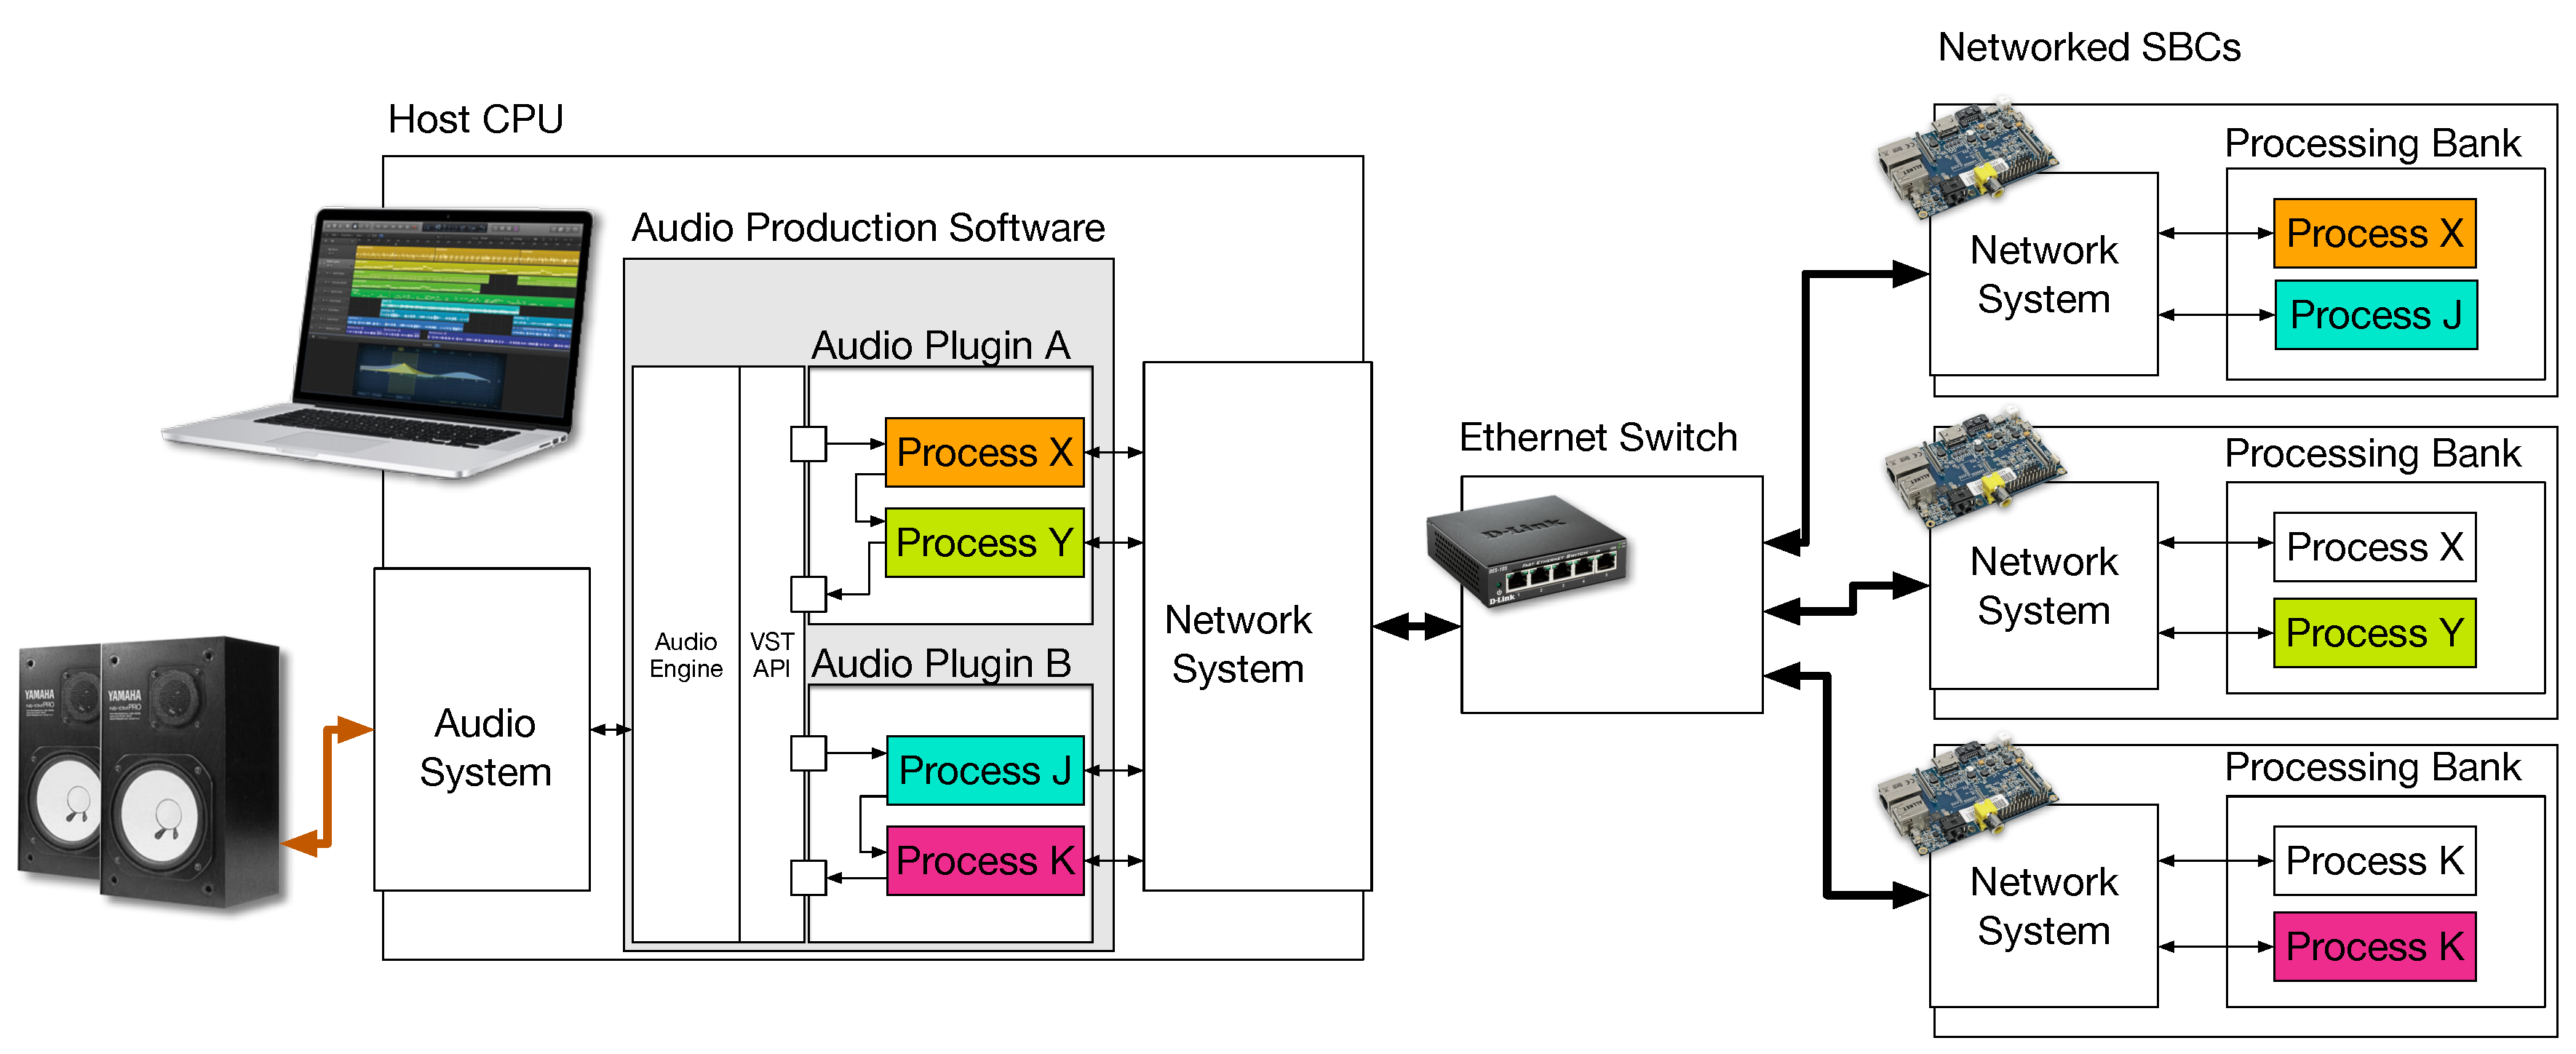
\includegraphics[width=\textwidth]{assets/architecture_01.pdf}
    \caption{Architektonischer Überblick}
    \label{fig:arch_01}
\end{figure}
